\section{Prueba 4: criterios adicionales al desempeño}
\subsection{Descripción} Se examinaron la equivalencia práctica, el costo, la estabilidad, la robustez y la interpretabilidad para complementar la exactitud. La hipótesis de equivalencia se evaluó con un margen de 0.03, sin interpretar la ausencia de significación como equivalencia.
\subsection{Procedimiento} Se aplicó la prueba bayesiana de rangos con signo sobre las medias por sujeto de las semillas 2026, 2027 y 2028, y se comparó con TOST; el detalle y las condiciones de cómputo se presentan en la sección~\ref{sec:estadistica}. La robustez y la saliencia se evaluaron con los pesos de 44 sujetos sobre los 10 apartados, con la semilla 2026. EEGMamba se excluyó de ambos análisis por no estar disponible \texttt{mamba\_ssm} en el entorno de inferencia.
\subsection{Resultados y análisis}
\begin{table}[htbp]\centering\small
\caption{Exactitud \loso{}: probabilidades posteriores para 54 sujetos y media de tres semillas. A y B siguen el orden del par; una decisión requiere probabilidad al menos 0.95.}
\resizebox{\textwidth}{!}{%
\begin{tabular}{lllll}
\toprule
Par A--B & P(A mejor) & P(equivalentes) & P(B mejor) & Decisión \\
\midrule
eegnet-conformer & 0.000 & 1.000 & 0.000 & equivalentes \\
eegnet-labram & 0.000 & 1.000 & 0.000 & equivalentes \\
conformer-labram & 0.000 & 0.999 & 0.001 & equivalentes \\
eegnet-eegmamba & 0.980 & 0.020 & 0.000 & A mejor \\
conformer-eegmamba & 0.864 & 0.136 & 0.000 & indeciso \\
labram-eegmamba & 0.983 & 0.017 & 0.000 & A mejor \\
\bottomrule\end{tabular}}\end{table}
\begin{table}[htbp]\centering\small
\caption{Exactitud intra-sujeto: probabilidades posteriores para 54 sujetos y media de tres semillas. A y B siguen el orden del par; una decisión requiere probabilidad al menos 0.95.}
\resizebox{\textwidth}{!}{%
\begin{tabular}{lllll}
\toprule
Par A--B & P(A mejor) & P(equivalentes) & P(B mejor) & Decisión \\
\midrule
eegnet-conformer & 0.811 & 0.189 & 0.000 & indeciso \\
eegnet-labram & 0.129 & 0.012 & 0.858 & indeciso \\
conformer-labram & 0.000 & 0.011 & 0.989 & B mejor \\
eegnet-eegmamba & 1.000 & 0.000 & 0.000 & A mejor \\
conformer-eegmamba & 0.310 & 0.690 & 0.000 & indeciso \\
labram-eegmamba & 0.999 & 0.001 & 0.000 & A mejor \\
\bottomrule\end{tabular}}\end{table}
\begin{table}[htbp]\centering\small
\caption{Degradación vistos menos no vistos: probabilidades posteriores para 54 sujetos y media de tres semillas. A y B siguen el orden del par; una decisión requiere probabilidad al menos 0.95.}
\resizebox{\textwidth}{!}{%
\begin{tabular}{lllll}
\toprule
Par A--B & P(A mejor) & P(equivalentes) & P(B mejor) & Decisión \\
\midrule
eegnet-conformer & 0.000 & 1.000 & 0.000 & equivalentes \\
eegnet-labram & 0.028 & 0.972 & 0.000 & equivalentes \\
conformer-labram & 0.006 & 0.994 & 0.000 & equivalentes \\
eegnet-eegmamba & 0.000 & 1.000 & 0.000 & equivalentes \\
conformer-eegmamba & 0.000 & 0.999 & 0.001 & equivalentes \\
labram-eegmamba & 0.000 & 0.998 & 0.002 & equivalentes \\
\bottomrule\end{tabular}}\end{table}
En degradación, una caída menor se consideró mejor. Los márgenes 0.01 y 0.02 modificaron las decisiones, por lo que la equivalencia depende del margen elegido. La comparación con TOST se presenta en la sección~\ref{sec:comparacion}.

Para la degradación, con 54 sujetos y media de tres semillas, TOST de Wilcoxon con Holm declaró equivalencia en los seis pares para el margen 0.03, en concordancia con la prueba bayesiana. Para \eegnet{}--LaBraM, la diferencia media fue $-0.021$, el intervalo percentil de remuestreo del 90\% fue $[-0.031, -0.012]$ y $p$ ajustado fue $0.026$; este intervalo rebasa el margen, aunque TOST declara equivalencia. Con ROPE 0.01 ningún par alcanzó probabilidad de equivalencia de 0.95; con ROPE 0.02 solo \eegnet{}--Conformer la alcanzó ($0.981$).
\begin{table}[htbp]\centering\small
\caption{Costo de inferencia con 62 canales. Latencias medianas en ms para lote 1; memoria pico CUDA en MB para lote 64. El contador cubre las operaciones compatibles.}
\resizebox{\textwidth}{!}{%
\begin{tabular}{lllllll}
\toprule
Arquitectura & Parámetros & FLOP/ensayo & CPU & CUDA & Memoria & Tamaño MB \\
\midrule
eegnet & 2898 & 52715968 & 2.09 & 0.67 & 218.25 & 0.07 \\
conformer & 710146 & 262463072 & 7.56 & 8.59 & 1019.07 & 8.37 \\
labram & 5818138 & 3469940000 & 34.04 & 10.61 & 477.61 & 70.20 \\
eegmamba & 3376445 & -- & -- & -- & -- & 40.40 \\
\bottomrule\end{tabular}}\end{table}
Para EEGMamba se informó el número de parámetros; las demás mediciones no estuvieron disponibles por la dependencia \texttt{mamba\_ssm}.
\begin{table}[htbp]\centering\small
\caption{Horas de entrenamiento: suma por ejecución, no tiempo de pared.}
\resizebox{\textwidth}{!}{%
\begin{tabular}{lllll}
\toprule
Arquitectura & Protocolo & Semilla & GPU & Horas \\
\midrule
eegnet & intra & 2026 & A40 & 1.31 \\
eegnet & intra & 2027 & A40 & 1.28 \\
eegnet & intra & 2028 & A40 & 1.26 \\
eegnet & \loso{} & 2026 & A40 & 6.69 \\
eegnet & \loso{} & 2027 & L40S & 6.62 \\
eegnet & \loso{} & 2028 & L40S & 7.26 \\
conformer & intra & 2026 & A40 & 1.37 \\
conformer & intra & 2027 & A40 & 1.38 \\
conformer & intra & 2028 & A40 & 1.36 \\
conformer & \loso{} & 2026 & A40 & 6.14 \\
conformer & \loso{} & 2027 & L40S & 8.52 \\
conformer & \loso{} & 2028 & L40S & 8.90 \\
labram & intra & 2026 & A40 & 6.67 \\
labram & intra & 2027 & L40S & 18.86 \\
labram & intra & 2028 & L40S & 18.96 \\
labram & \loso{} & 2026 & A40 & 21.30 \\
labram & \loso{} & 2027 & L40S & 34.47 \\
labram & \loso{} & 2028 & L40S & 34.22 \\
eegmamba & intra & 2026 & A40 & 10.99 \\
eegmamba & intra & 2027 & L40S & 5.05 \\
eegmamba & intra & 2028 & L40S & 4.93 \\
eegmamba & \loso{} & 2026 & A40 & 24.98 \\
eegmamba & \loso{} & 2027 & L40S & 16.84 \\
eegmamba & \loso{} & 2028 & L40S & 16.65 \\
\bottomrule\end{tabular}}\end{table}
\begin{table}[htbp]\centering\small
\caption{Estabilidad sobre 54 sujetos: desviación entre medias de semilla, tau de Kendall y porcentaje de signo consistente frente a EEGNet.}
\resizebox{\textwidth}{!}{%
\begin{tabular}{llllll}
\toprule
Protocolo & Arquitectura & Semillas & DE & Tau & Signo (\%) \\
\midrule
within & eegnet & 2026-2027-2028 & 0.004 & 0.767 & -- \\
within & eegnet & 2027-2028 & 0.006 & 0.746 & -- \\
within & conformer & 2026-2027-2028 & 0.004 & 0.769 & 68.52 \\
within & conformer & 2027-2028 & 0.000 & 0.757 & 79.63 \\
within & labram & 2026-2027-2028 & 0.001 & 0.833 & 79.63 \\
within & labram & 2027-2028 & 0.001 & 0.842 & 81.48 \\
within & eegmamba & 2026-2027-2028 & 0.006 & 0.547 & 75.93 \\
within & eegmamba & 2027-2028 & 0.005 & 0.589 & 85.19 \\
loso & eegnet & 2026-2027-2028 & 0.002 & 0.836 & -- \\
loso & eegnet & 2027-2028 & 0.000 & 0.816 & -- \\
loso & conformer & 2026-2027-2028 & 0.004 & 0.786 & 50.00 \\
loso & conformer & 2027-2028 & 0.000 & 0.756 & 66.67 \\
loso & labram & 2026-2027-2028 & 0.002 & 0.786 & 40.74 \\
loso & labram & 2027-2028 & 0.003 & 0.797 & 66.67 \\
loso & eegmamba & 2026-2027-2028 & 0.001 & 0.819 & 64.81 \\
loso & eegmamba & 2027-2028 & 0.001 & 0.814 & 74.07 \\
\bottomrule\end{tabular}}\end{table}
\begin{table}[htbp]\centering\small
\caption{Caída de exactitud e intervalo del 95\% ante perturbaciones; 10 sujetos apartados y semilla 2026.}
\resizebox{\textwidth}{!}{%
\begin{tabular}{lllll}
\toprule
Arquitectura & Perturbación & Nivel & Caída & IC 95\% \\
\midrule
conformer & canales & 0.10 & 0.036 & [0.021, 0.053] \\
conformer & canales & 0.20 & 0.068 & [0.042, 0.097] \\
conformer & canales & 0.30 & 0.103 & [0.066, 0.141] \\
conformer & desplazamiento\_s & 0.10 & 0.000 & [-0.005, 0.006] \\
conformer & desplazamiento\_s & 0.25 & 0.023 & [0.011, 0.033] \\
conformer & desplazamiento\_s & 0.50 & 0.053 & [0.030, 0.076] \\
conformer & escala & 0.50 & 0.039 & [0.007, 0.072] \\
conformer & escala & 2.00 & -0.004 & [-0.018, 0.009] \\
conformer & red & 0.10 & -0.000 & [-0.001, 0.001] \\
conformer & red & 0.50 & -0.003 & [-0.008, 0.001] \\
conformer & ruido\_db & 0.00 & 0.064 & [0.045, 0.084] \\
conformer & ruido\_db & 5.00 & 0.019 & [0.006, 0.031] \\
conformer & ruido\_db & 10.00 & 0.000 & [-0.006, 0.007] \\
conformer & ruido\_db & 20.00 & -0.002 & [-0.005, 0.000] \\
eegnet & canales & 0.10 & 0.047 & [0.028, 0.067] \\
eegnet & canales & 0.20 & 0.081 & [0.050, 0.114] \\
eegnet & canales & 0.30 & 0.118 & [0.082, 0.157] \\
eegnet & desplazamiento\_s & 0.10 & 0.009 & [-0.000, 0.021] \\
eegnet & desplazamiento\_s & 0.25 & 0.047 & [0.025, 0.071] \\
eegnet & desplazamiento\_s & 0.50 & 0.080 & [0.048, 0.113] \\
eegnet & escala & 0.50 & 0.013 & [-0.010, 0.038] \\
eegnet & escala & 2.00 & 0.019 & [0.002, 0.036] \\
eegnet & red & 0.10 & 0.000 & [-0.001, 0.002] \\
eegnet & red & 0.50 & 0.005 & [-0.002, 0.012] \\
eegnet & ruido\_db & 0.00 & 0.071 & [0.049, 0.094] \\
eegnet & ruido\_db & 5.00 & 0.030 & [0.017, 0.044] \\
eegnet & ruido\_db & 10.00 & 0.012 & [0.004, 0.020] \\
eegnet & ruido\_db & 20.00 & 0.002 & [-0.001, 0.005] \\
labram & canales & 0.10 & 0.017 & [0.009, 0.025] \\
labram & canales & 0.20 & 0.042 & [0.027, 0.059] \\
labram & canales & 0.30 & 0.070 & [0.047, 0.093] \\
labram & desplazamiento\_s & 0.10 & 0.008 & [-0.002, 0.018] \\
labram & desplazamiento\_s & 0.25 & 0.035 & [0.021, 0.048] \\
labram & desplazamiento\_s & 0.50 & 0.082 & [0.053, 0.111] \\
labram & escala & 0.50 & 0.003 & [-0.002, 0.007] \\
labram & escala & 2.00 & -0.001 & [-0.004, 0.003] \\
labram & red & 0.10 & 0.001 & [-0.000, 0.002] \\
labram & red & 0.50 & 0.002 & [-0.001, 0.006] \\
labram & ruido\_db & 0.00 & 0.076 & [0.054, 0.097] \\
labram & ruido\_db & 5.00 & 0.038 & [0.026, 0.051] \\
labram & ruido\_db & 10.00 & 0.014 & [0.006, 0.024] \\
labram & ruido\_db & 20.00 & 0.002 & [-0.002, 0.008] \\
\bottomrule\end{tabular}}\end{table}
\begin{table}[htbp]\centering\small
\caption{Índices de lateralización para 10 sujetos apartados y semilla 2026.}
\resizebox{\textwidth}{!}{%
\begin{tabular}{llll}
\toprule
Arquitectura & Clase & C3/C4 & Vecindad \\
\midrule
eegnet & izquierda & -0.086 & 0.045 \\
eegnet & derecha & -0.001 & 0.127 \\
conformer & izquierda & -0.005 & 0.065 \\
conformer & derecha & -0.021 & 0.077 \\
labram & izquierda & -0.004 & -0.006 \\
labram & derecha & 0.067 & 0.061 \\
\bottomrule\end{tabular}}\end{table}
No se observó un patrón contralateral uniforme. Los mapas describen sensibilidad de los modelos y no establecen causalidad. La eficiencia de datos se examinó mediante la calibración de la subsección~\ref{sec:fewshot}.
\begin{figure}[htbp]\centering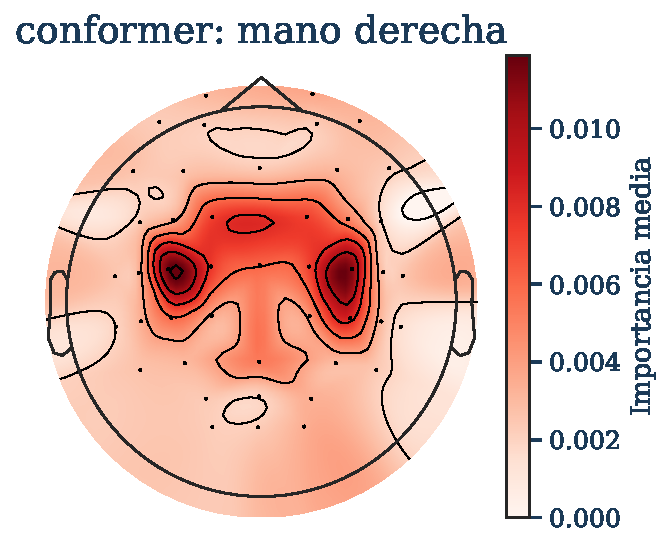
\includegraphics[width=0.65\textwidth]{figuras/interp_conformer_derecha.pdf}\caption{Sensibilidad espacial o filtros: interp conformer derecha; 10 sujetos apartados, semilla 2026.}\end{figure}
\begin{figure}[htbp]\centering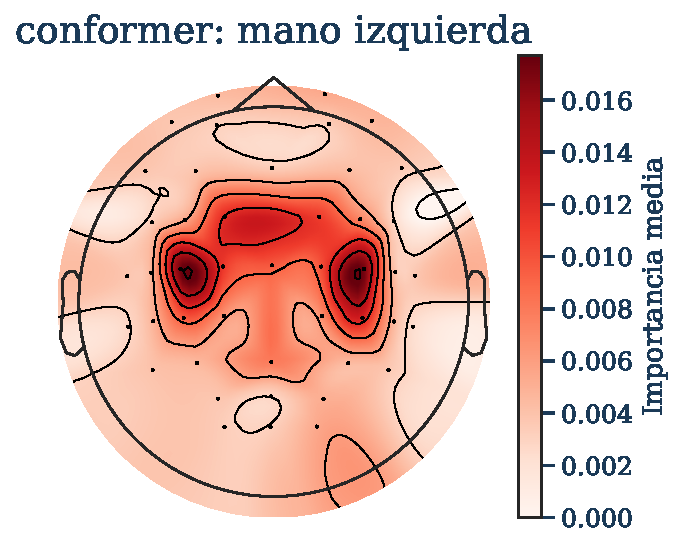
\includegraphics[width=0.65\textwidth]{figuras/interp_conformer_izquierda.pdf}\caption{Sensibilidad espacial o filtros: interp conformer izquierda; 10 sujetos apartados, semilla 2026.}\end{figure}
\begin{figure}[htbp]\centering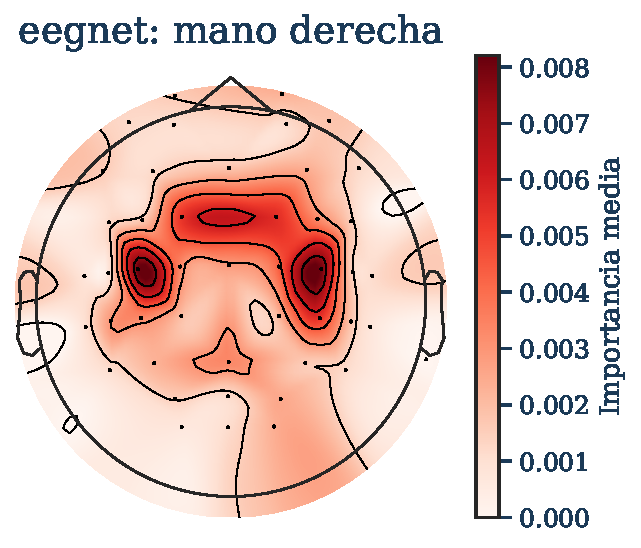
\includegraphics[width=0.65\textwidth]{figuras/interp_eegnet_derecha.pdf}\caption{Sensibilidad espacial o filtros: interp eegnet derecha; 10 sujetos apartados, semilla 2026.}\end{figure}
\begin{figure}[htbp]\centering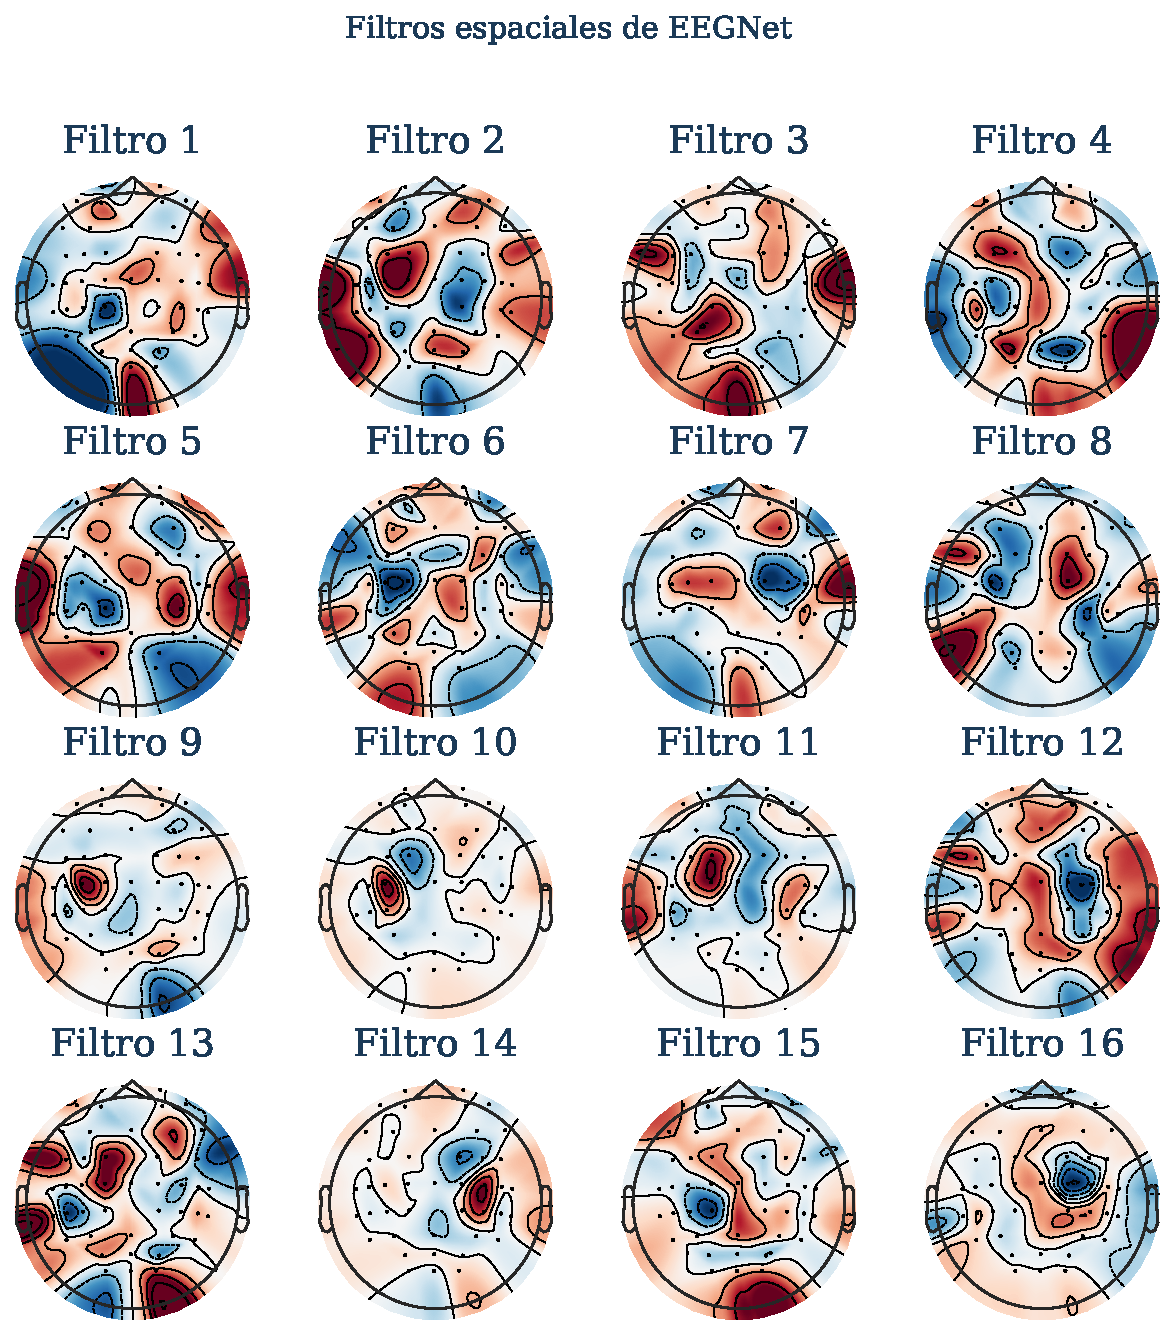
\includegraphics[width=0.65\textwidth]{figuras/interp_eegnet_filtros.pdf}\caption{Sensibilidad espacial o filtros: interp eegnet filtros; 10 sujetos apartados, semilla 2026.}\end{figure}
\begin{figure}[htbp]\centering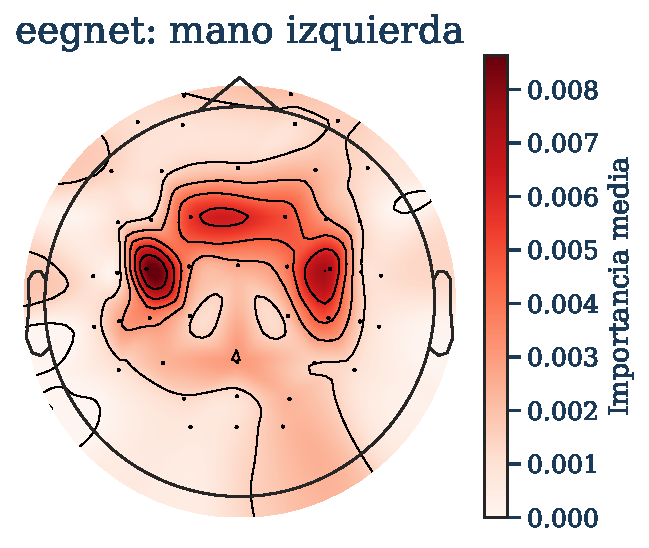
\includegraphics[width=0.65\textwidth]{figuras/interp_eegnet_izquierda.pdf}\caption{Sensibilidad espacial o filtros: interp eegnet izquierda; 10 sujetos apartados, semilla 2026.}\end{figure}
\begin{figure}[htbp]\centering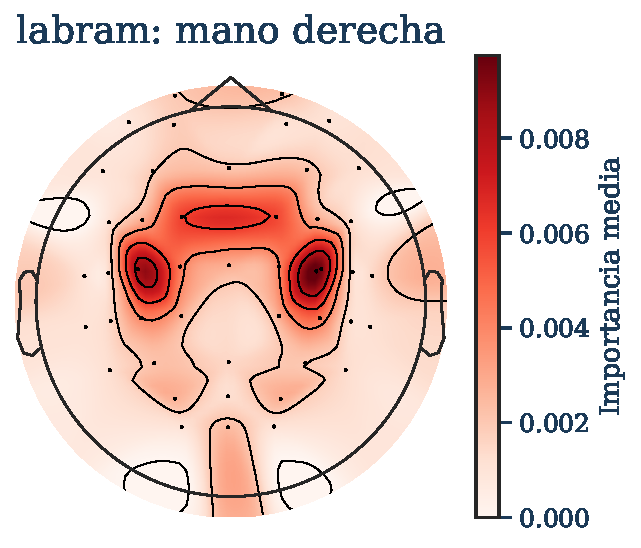
\includegraphics[width=0.65\textwidth]{figuras/interp_labram_derecha.pdf}\caption{Sensibilidad espacial o filtros: interp labram derecha; 10 sujetos apartados, semilla 2026.}\end{figure}
\begin{figure}[htbp]\centering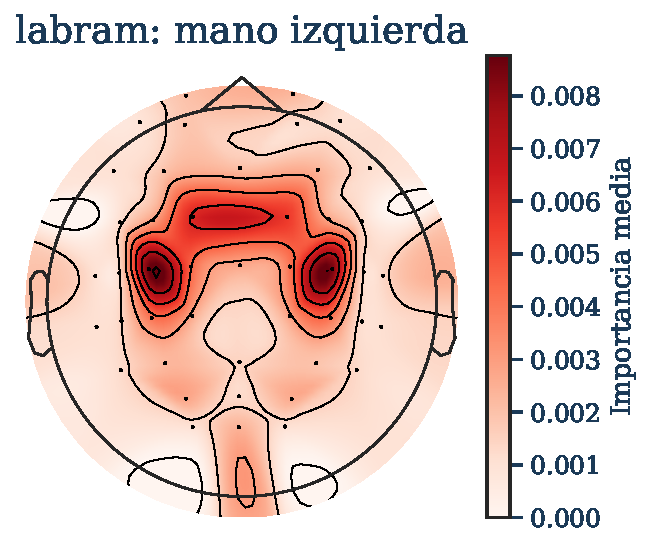
\includegraphics[width=0.65\textwidth]{figuras/interp_labram_izquierda.pdf}\caption{Sensibilidad espacial o filtros: interp labram izquierda; 10 sujetos apartados, semilla 2026.}\end{figure}
